\documentclass[12pt]{article}
%\usepackage[a4paper,width=150mm,top=10mm,bottom=20mm]{geometry}
\usepackage[a4paper,width=160mm,top=25mm,bottom=25mm]{geometry}



%%%%% For Title Page %%%%%
\usepackage{graphicx}
\usepackage{subcaption}
\usepackage{etoolbox}
\usepackage{relsize}
%%%%%%%%%%%%%%%%%%%%%%%%%%

\usepackage[utf8]{inputenc}





% Redéfinition des marques pour utiliser la section et la sous-section
\renewcommand{\sectionmark}[1]{\markboth{#1}{}}
\renewcommand{\subsectionmark}[1]{\markright{\thesubsection\ #1}}



\newcommand{\nsection}[1]{%
  \section*{#1}%
  \addcontentsline{toc}{section}{#1}%
  \markboth{#1}{}% Met à jour les deux marques pour les sections non numérotées
  
}

\newcommand{\nsubsection}[1]{%
  \subsection*{#1}%
  \addcontentsline{toc}{subsection}{#1}%
  \markright{#1}% Met à jour la marque de droite pour les sous-sections non numérotées
}




\usepackage[utf8]{inputenc}
\usepackage[T1]{fontenc}
\usepackage[french]{babel}
\usepackage{titling}
\usepackage{graphicx}
\usepackage{svg}
% Ajouter dans le préambule du document :
\usepackage{minted}
\usepackage{xcolor}
\usepackage{float}
\floatplacement{figure}{H}
\usepackage[colorlinks=true, linkcolor=blue]{hyperref}
\usepackage[all]{hypcap}
\usepackage{amsmath}
\usepackage{fancyhdr}
\usepackage{lastpage}



%\geometry{margin=2.5cm}
\setlength{\headheight}{15pt}

% Configuration de fancyhdr

\fancyhf{} % Efface tous les champs d'en-tête et de pied de page
\renewcommand{\headrulewidth}{0.4pt} % Ajoute une ligne d'en-tête

% Configuration de l'en-tête pour les pages normales
\fancyhead[L]{\leftmark}
\fancyhead[R]{\rightmark}

% Configuration pour la première page
\fancypagestyle{plain}{
    \fancyhf{} % Efface les en-têtes et pieds de page par défaut
}


    
\begin{document} 

\newcommand{\anneeuniv}{2024--2025}
\newcommand{\master}{Master 1 TDSI - parcours Objets Connectés}
\newcommand{\titre}{Station Météo}
\renewcommand{\author}{GROUSSARD Tristan \& DJESSOU Koundeme Nobel \& MORET Maxime}
\newcommand{\teacher}{BOEGLEN Hervé \& RICHARD Noel}



\thispagestyle{empty}


\begin{titlepage}

\newgeometry{width=160mm,top=10mm,bottom=20mm}

  \begingroup

\begin{figure}[H]
  \centering
  \begin{minipage}{.5\textwidth}
    \flushleft
    
\includegraphics[height=80pt]{figs/Logo-up.pdf}
  \end{minipage}%
  \begin{minipage}{.5\textwidth}
    \flushright
    
\includegraphics[height=80pt]{figs/Logo-moc.png}
  \end{minipage}
\end{figure}

  
  \hrulefill

  \begin{center}
      \vspace{-0.5cm}
      Université de Poitiers, Année universitaire \anneeuniv\\
      U.F.R. Sciences Fondamentales Appliquées\\
      \master
  \end{center}
  
   \vspace{-3cm}

  \vfill
  
  \begin{center}
    {\huge\textbf{\titre}}\\
    \vspace{1.25cm}
    {\large Projet Module Systèmes Embarqués 2024}\\
    \vspace{3.5cm}
    \author\\
  \end{center}

  \vfill

  \hrulefill
  \flushright
  \vspace{-0.3cm}
  
  \ifdefempty{\teacher}{}{Module enseigné par \teacher\\}

  \endgroup

\restoregeometry
  
\end{titlepage}




\pagenumbering{gobble}


\tableofcontents
\label{toc} % Étiquette pour le lien


\listoffigures

\newpage


\clearpage
\setcounter{page}{3}
\pagenumbering{arabic}
\fancyfoot[C]{\hyperlink{toc}{\thepage} / \pageref{LastPage}} % Numéro de page au centre avec total
 %\fancyfoot[R]{\hyperlink{toc}{\thepage}}

\pagestyle{fancy}

\nsection{Introduction}
Le réchauffement climatique est un des défis majeurs auquel l'humanité aura à faire face dans les prochaines années. L'influence de l'activité humaine, longtemps contestée, ne fait plus aucun doute. D'après un récent rapport de l'Organisation Météorologique Mondiale, 2019 est la 5\textsuperscript{ème} année la plus chaude depuis le début des relevés météorologiques en 1850. La température moyenne en 2018 est de 1°C supérieure à celle relevée à l'ère préindustrielle.

Selon les travaux des scientifiques du GIEC, si l'humanité veut continuer à vivre sur la planète sans subir des changements climatiques catastrophiques mettant en cause sa survie et celle de tous les êtres vivants, cette température moyenne ne devra pas excéder 1.5°C d'ici à la fin de ce siècle.

Dans ce contexte, il est intéressant de pouvoir disposer d'un équipement permettant de relever les différentes grandeurs météorologiques du lieu où l'on se trouve.

L'objectif de ce projet, utilisant un système embarqué, est donc de concevoir et de réaliser une station météorologique.

\section{Cahier des charges}
\subsection{Objectifs détaillés}
L'objectif de ce projet est de réaliser une station météorologique utilisant une carte STM32F746G DIscovery.
Cette station doit etre capable de mesurer : 
\begin{itemize}
    \item La température
    \item La pression atmosphérique
    \item L'humidité
    \item La luminosité
    \item La direction et la vitesse du vent
    \item La quantité d'eau tombée en une journée (pluviométrie)
\end{itemize}
Ces mesures seront affichées et stockées directement sur la station (en utilisant le LCD et le lecteur de carte SD de la carte Discovery) et pourront également être transmises par radio vers un dispositif distant (smartphone, Raspberry Pi, etc.).


\subsection{Table des Entrées/Sorties}
\begin{table}[H]
    \centering
    \caption{Table des Entrées/Sorties du système}
    \begin{tabular}{|l|l|l|l|l|}
    \hline
    \textbf{Composant} & \textbf{Type} & \textbf{Interface} & \textbf{Pins STM32} & \textbf{Caractéristiques} \\
    \hline
    HTS221 & Entrée & I2C1 & 
    \begin{tabular}[c]{@{}l@{}}
    PB8 (SCL)\\
    PB9 (SDA)
    \end{tabular} & 
    \begin{tabular}[c]{@{}l@{}}
    Humidité: 0-100\%\\
    Temp: -40 à +120°C
    \end{tabular} \\
    \hline
    LPS22HH & Entrée & I2C1 & 
    \begin{tabular}[c]{@{}l@{}}
    PB8 (SCL)\\
    PB9 (SDA)
    \end{tabular} & 
    Pression: 260-1260 hPa \\
    \hline
    Anémomètre & Entrée & GPIO & PC6 & 2,4km/h = 1Hz \\
    \hline
    Girouette & Entrée & ADC & PA8 & 16 positions (0-360°) \\
    \hline
    Pluviomètre & Entrée & GPIO & PA15 & 0,2794mm/impulsion \\
    \hline
    Écran LCD & Sortie & LTDC & 
    \begin{tabular}[c]{@{}l@{}}
    Multiple pins\\
    (voir datasheet)
    \end{tabular} & 480x272 pixels \\
    \hline
    Carte SD & E/S & SDIO & 
    \begin{tabular}[c]{@{}l@{}}
    PC8-PC11\\
    (données)\\
    PC12 (CLK)\\
    PD2 (CMD)
    \end{tabular} & Mode 4-bits \\
    \hline
    \end{tabular}
\end{table}
    

\subsection{Spécifications fonctionnelles}

La station météorologique doit répondre aux fonctionnalités suivantes :

\subsubsection{Acquisition des données}
\begin{itemize}
    \item Mesure de la température ambiante (plage de -40°C à +120°C)
    \item Mesure du taux d'humidité relative (0-100\%)
    \item Mesure de la pression atmosphérique (260-1260 hPa)
    \item Mesure de la vitesse du vent (conversion 2,4 km/h = 1 Hz)
    \item Mesure de la direction du vent (16 positions sur 360°)
    \item Mesure de la pluviométrie (résolution de 0,2794 mm par basculement)
\end{itemize}

\subsubsection{Traitement et stockage}
\begin{itemize}
    \item Calcul des moyennes sur différentes périodes (horaire, journalière)
    \item Détection des valeurs extrêmes (minimum et maximum)
    \item Stockage des données sur carte SD
    \begin{itemize}
        \item Format de fichier structuré pour exploitation ultérieure
        \item Horodatage de chaque mesure
        \item Organisation par jour/mois
    \end{itemize}
    \item Conservation de l'historique des mesures
\end{itemize}

\subsubsection{Interface utilisateur}
\begin{itemize}
    \item Affichage en temps réel sur écran LCD 480x272 pixels
    \begin{itemize}
        \item Valeurs courantes des capteurs
        \item Graphiques d'évolution
    \end{itemize}
    \item Navigation entre différents écrans
    \begin{itemize}
        \item Écran principal des mesures
        \item Écrans détaillés par type de mesure
        \item Écran de configuration
        \item Écran des graphiques
    \end{itemize}
    \item Configuration système
    \begin{itemize}
        \item Réglage date et heure
    \end{itemize}
\end{itemize}

\subsubsection{Gestion de l'énergie}
\begin{itemize}
    \item Optimisation de la consommation énergétique
    \item Adaptation de la fréquence d'échantillonnage selon les besoins
    \item Utilisation des modes basse consommation lorsque possible
\end{itemize}

\subsubsection{Communication}
\begin{itemize}
    \item Transmission des données vers un dispositif distant
    \item Possibilité de configuration à distance
    \item Remontée des alertes en cas de dépassement de seuils
\end{itemize}


\section{Analyse technique des composants}
\subsection{Caractéristiques du shield ST X-NUCLEO-IKS01A3}
\begin{itemize}
    \item \textbf{LSM6DSO}: Accéléromètre 3D ($\pm2/\pm4/\pm8/\pm16g$) et gyroscope 3D ($\pm125/\pm250/\pm500/\pm1000/\pm2000$ dps)
    \item \textbf{LIS2MDL}: Magnétomètre 3D ($\pm50$ gauss)
    \item \textbf{LIS2DW12}: Accéléromètre 3D ($\pm2/\pm4/\pm8/\pm16g$)
    \item \textbf{LPS22HH}: Capteur de pression (baromètre à sortie numérique absolue de 260-1260 hPa)
    \item \textbf{HTS221}: Capteur d'humidité relative et de température
    \item \textbf{STTS751}: Capteur de température (plage de $-40°C$ à $+125°C$)
\end{itemize}

\subsection{Étude des capteurs}
\subsubsection{Température, humidité et pression}
La récupération des données des capteurs sur la carte d'extension \textbf{X-NUCLEO-IKS01A3} se fait principalement via le bus \textbf{I2C} (Inter-Integrated Circuit).

\subsection*{Configurations possibles}

La carte peut être configurée de deux manières différentes pour la communication I2C :
\begin{itemize}
    \item \textbf{Mode standard} : Tous les capteurs sont connectés sur un seul bus I2C.
    \item \textbf{Mode SensorHub} :
    \begin{itemize}
        \item \textbf{LSM6DSO} et \textbf{LIS2DW12} sont connectés au bus \textbf{I2C2}.
        \item Les autres capteurs (\textbf{LIS2MDL}, \textbf{LPS22HH}, \textbf{HTS221}, \textbf{STTS751}) sont connectés au \textbf{LSM6DSO} via le bus \textbf{I2C1}.
    \end{itemize}
\end{itemize}

Le choix du mode se fait par la configuration des cavaliers \textbf{JP7} et \textbf{JP8} sur la carte.

\subsection*{Particularités}

\begin{itemize}
    \item La carte s'interface avec les microcontrôleurs \textbf{STM32} via la broche \textbf{I2C1}.
    \item Il est possible de modifier le port I2C par défaut si nécessaire.
    \item Le \textbf{LSM6DSO} peut fonctionner comme un hub I2C pour les autres capteurs.
\end{itemize}

Cette flexibilité dans la configuration du bus I2C permet d'adapter la carte à différents besoins et scénarios d'utilisation.

\subsubsection{Anémomètre et girouette}
Le capteur de vitesse du vent, ou \textbf{anémomètre}, est de type à coupelles. Il mesure la vitesse du vent en fermant un contact lorsqu'un aimant passe devant un interrupteur. 
\begin{itemize}
    \item Une vitesse de vent de \textbf{2,4 km/h} provoque la fermeture de l'interrupteur une fois par seconde.
    \item L'interrupteur de l'anémomètre est connecté aux deux conducteurs intérieurs du câble \textbf{RJ11} partagé par l'anémomètre et la girouette (broches 2 et 3).
\end{itemize}

Le capteur de direction du vent, ou \textbf{girouette}, est le plus complexe des trois capteurs. 
\begin{itemize}
    \item Il possède huit interrupteurs, chacun connecté à une résistance différente.
    \item L'aimant de la girouette peut fermer deux interrupteurs à la fois, ce qui permet d'indiquer jusqu'à \textbf{16 positions différentes}.
    \item Une résistance externe peut être utilisée pour former un diviseur de tension, produisant une tension de sortie mesurable avec un convertisseur analogique-numérique.
\end{itemize}

Les valeurs de résistance pour toutes les 16 positions possibles sont données dans le tableau du document source. Les valeurs de résistance pour les positions intermédiaires sont le résultat de deux résistances adjacentes connectées en parallèle lorsque l'aimant de la girouette active deux interrupteurs simultanément.

\subsubsection{Pluviomètre}
Le capteur de pluie utilise le principe du \textbf{« tipping bucket »}, aussi appelé \textbf{auget basculeur}. Ce type de pluviomètre est constitué de deux petits récipients montés sur un axe horizontal. Lorsqu'un récipient est rempli par l'eau de pluie, il bascule sous son poids, vidant son contenu et permettant à l'autre récipient de se remplir. Chaque basculement ferme un contact électrique qui peut être enregistré par un compteur numérique ou une interruption de microcontrôleur.

\subsection*{Récupération des données de pluviométrie avec le STM32}

Pour récupérer l'information de pluviométrie avec le \textbf{STM32}, il faut :
\begin{itemize}
    \item Connecter l'interrupteur du pluviomètre aux deux conducteurs centraux d'un câble \textbf{RJ11}.
    \item Configurer une broche du \textbf{STM32} en entrée d'interruption pour détecter la fermeture du contact.
    \item Compter le nombre d'interruptions pour déterminer la quantité de pluie tombée.
\end{itemize}

Chaque basculement correspond à une quantité de pluie précise. Dans ce cas, chaque basculement de l'auget représente \textbf{0,2794 mm} de pluie.

\section{Analyse préliminaire}
Afin que tout fonctionne au mieux, on a eu plusieurs séances de travail en groupe pour bien comprendre le fonctionnement de chaque capteur et de la carte STM32F746G Discovery.
Voici les questions principales auxquelles on a répondu lors de ces séances de travail :
\begin{itemize}
    \item Comment fonctionne chaque capteur ?
    \item Comment sont-ils connectés à la carte STM32 ?
    \item Combien de timers seront utilsés? A quoi vont servir ces timers?
    \item Quelles sont les fonctionnalités nécessaires pour l'interface utilisateur?
    \item Comment stocker les données sur la carte SD?
    \item Que souhaite t-on afficher sur l'écran LCD?
    \item Comment gérer les interruptions pour les capteurs de vitesse et de pluie?
    \item Tout doit fonctionner à quelle fréquence?
    \item Quel sera la fréquence pour chaque timer?
    \item Comment gérer les erreurs?
\end{itemize}

Après avoir répondu à ces questions, nous avons défini le prototype de notre interface utilisateur :

\begin{figure}[H]
    \capstart
    \centering
    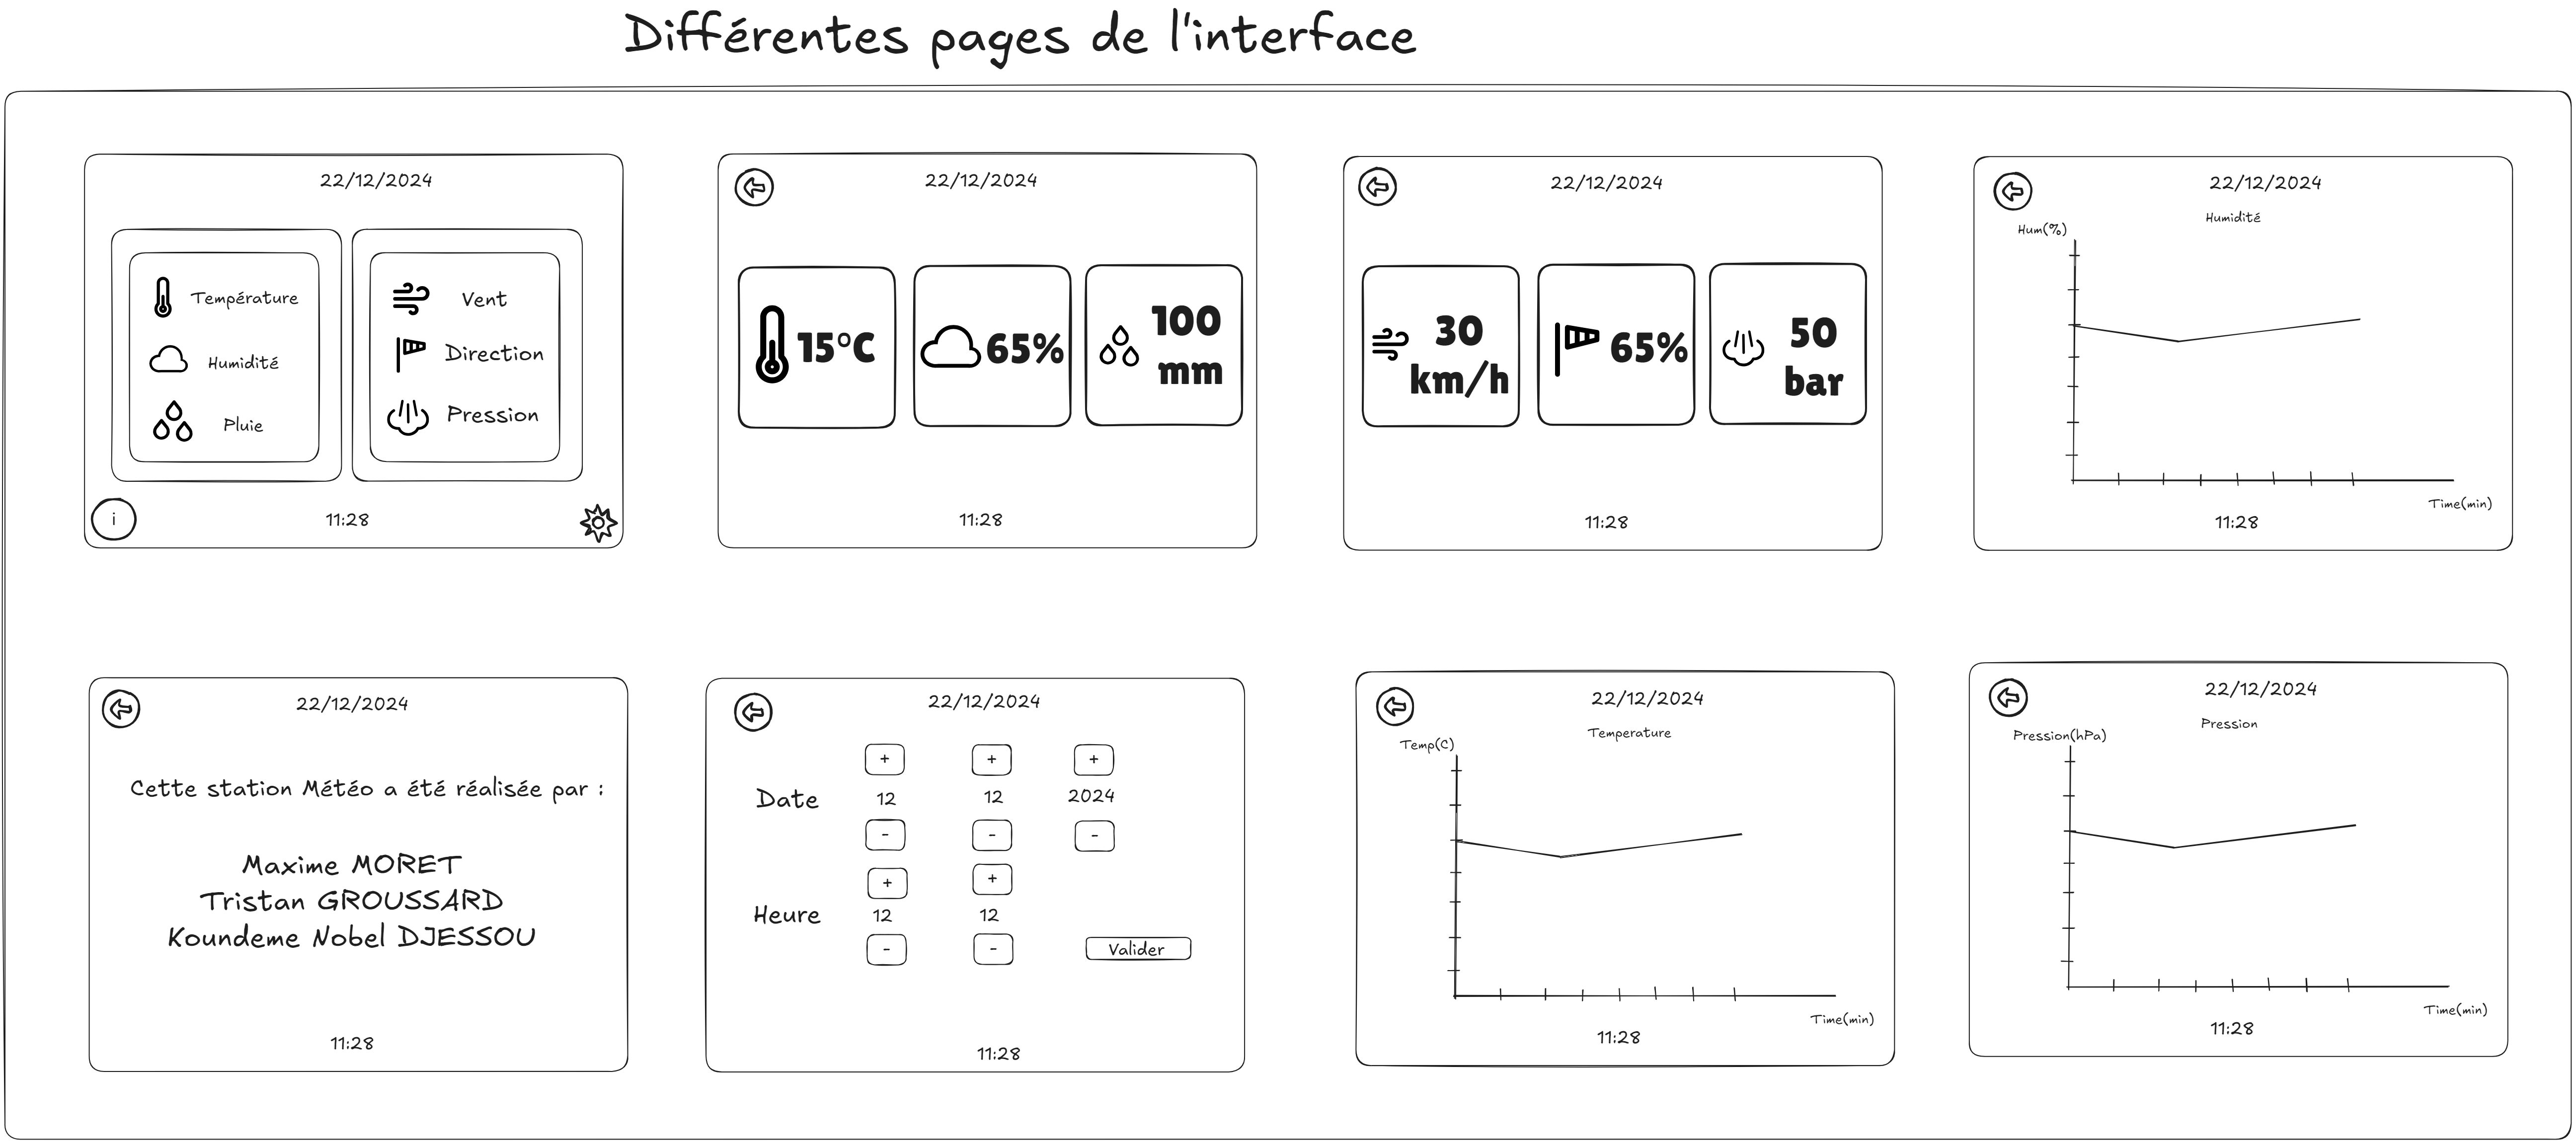
\includegraphics[width=0.8\textwidth]{./images/prototype_interface1.png}
    \caption{Interface utilisateur}
    \label{fig:interface}
\end{figure}

Notre interface utilisateur est divisée en cinq parties principales :
\begin{itemize}
    \item L'écran principal : affichage des grandeurs mesurées en temps réel
    \item Deux pages qui affichent les valeurs en temps réel des capteurs
    \item L'écran configuration qui permet de configurer la date et l'heure
    \item La page des informations qui affiche les informations sur le projet
    \item Les pages des graphiques(température,humidité,pression)
\end{itemize}

Une fois cette interface définie, nous avons pu commencer à travailler sur les différents diagrammes de flot de données, de flot d'événements et de GRAFCET.
\subsection{Organisation du système}
Le système peut être divisé en trois sous-systèmes principaux interagissant entre eux :
\begin{itemize}
    \item \textbf{Système d'acquisition} : gestion des capteurs et conversion des données
    \item \textbf{Système de traitement} : traitement des données et gestion des interruptions
    \item \textbf{Système d'interface} : affichage LCD et stockage SD
\end{itemize}

\subsection{Diagramme des bords du modèle}
Le diagramme des bords du modèle montre les interactions entre le STM32 et ses périphériques externes :

\begin{figure}[H]
    \capstart
    \centering
    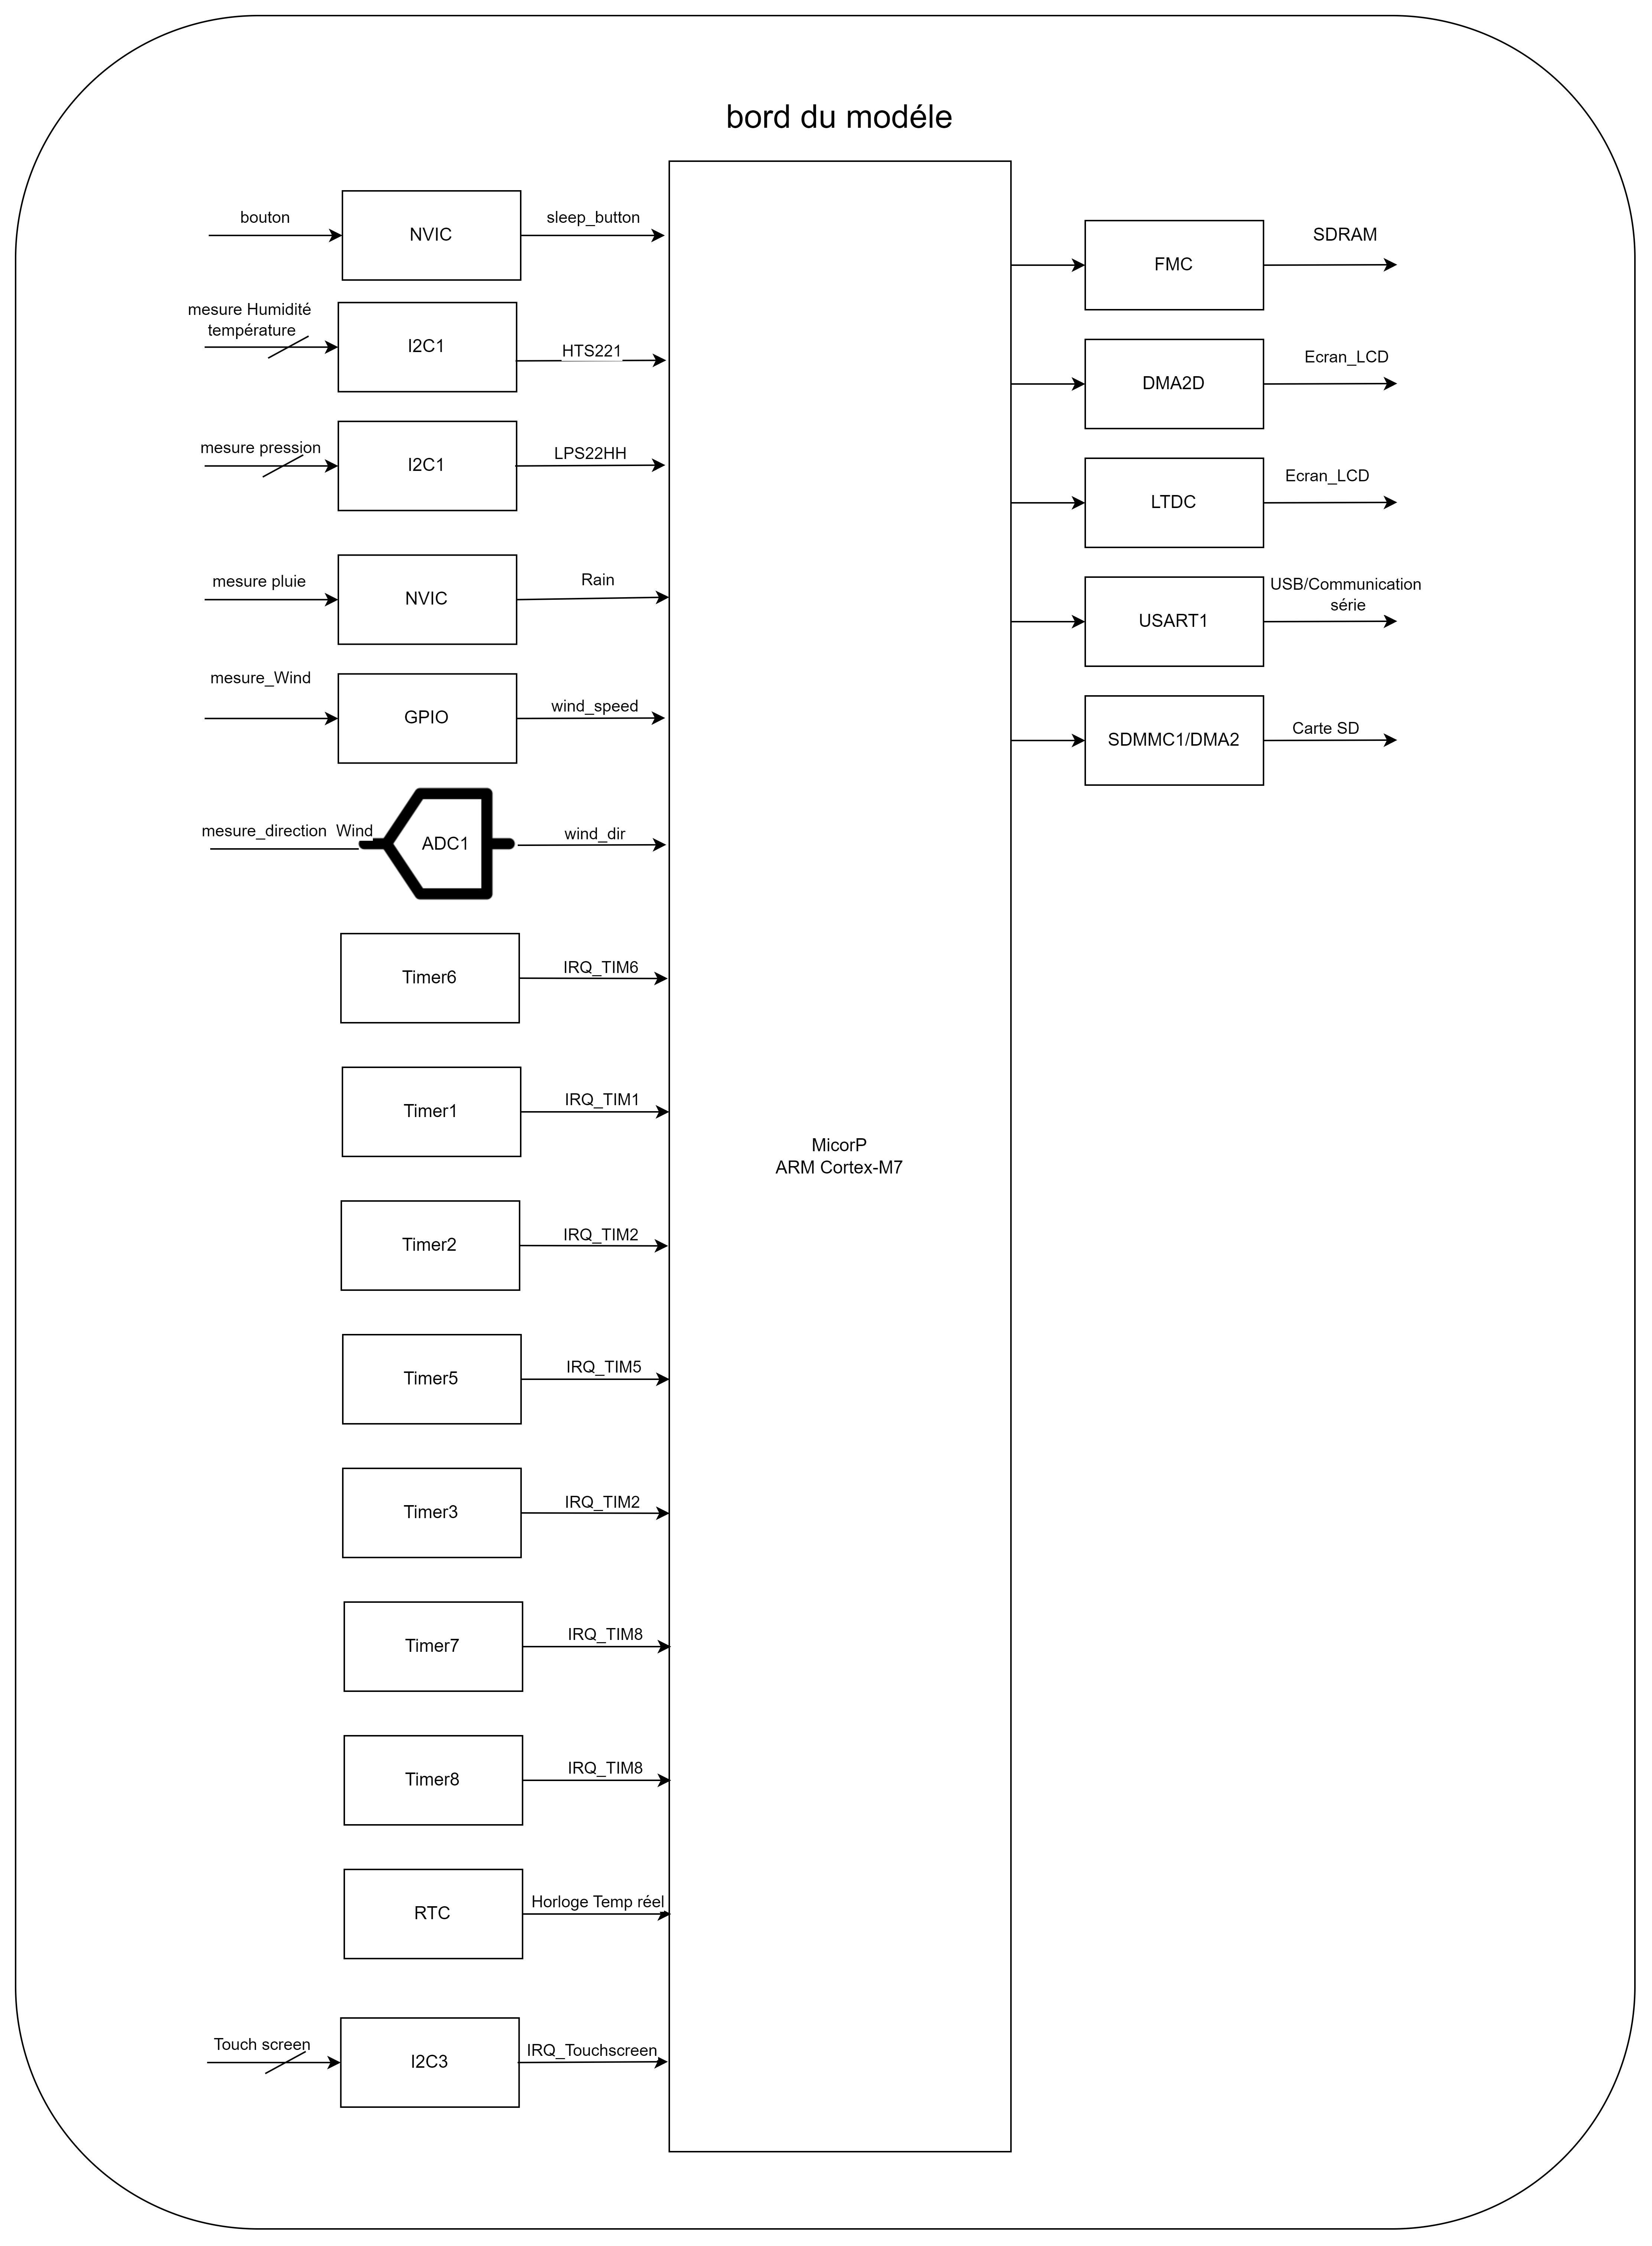
\includegraphics[width=0.8\textwidth]{./images/bords_du_modele1.png}
    \caption{Bords du modèle}
    \label{fig:bords}
\end{figure}

Les principaux éléments sont :
\begin{itemize}
    \item \textbf{Capteurs I2C} : HTS221 (température/humidité) et LPS22HH (pression)
    \item \textbf{Capteurs à impulsions} : anémomètre et pluviomètre
    \item \textbf{Capteur analogique} : girouette
    \item \textbf{Interface utilisateur} : écran LCD
    \item \textbf{Stockage} : carte SD
\end{itemize}

\subsection{Diagramme de flot de données}
Le diagramme de flot de données illustre le cheminement des données à travers le système :

\begin{figure}[H]
    \capstart
    \centering
    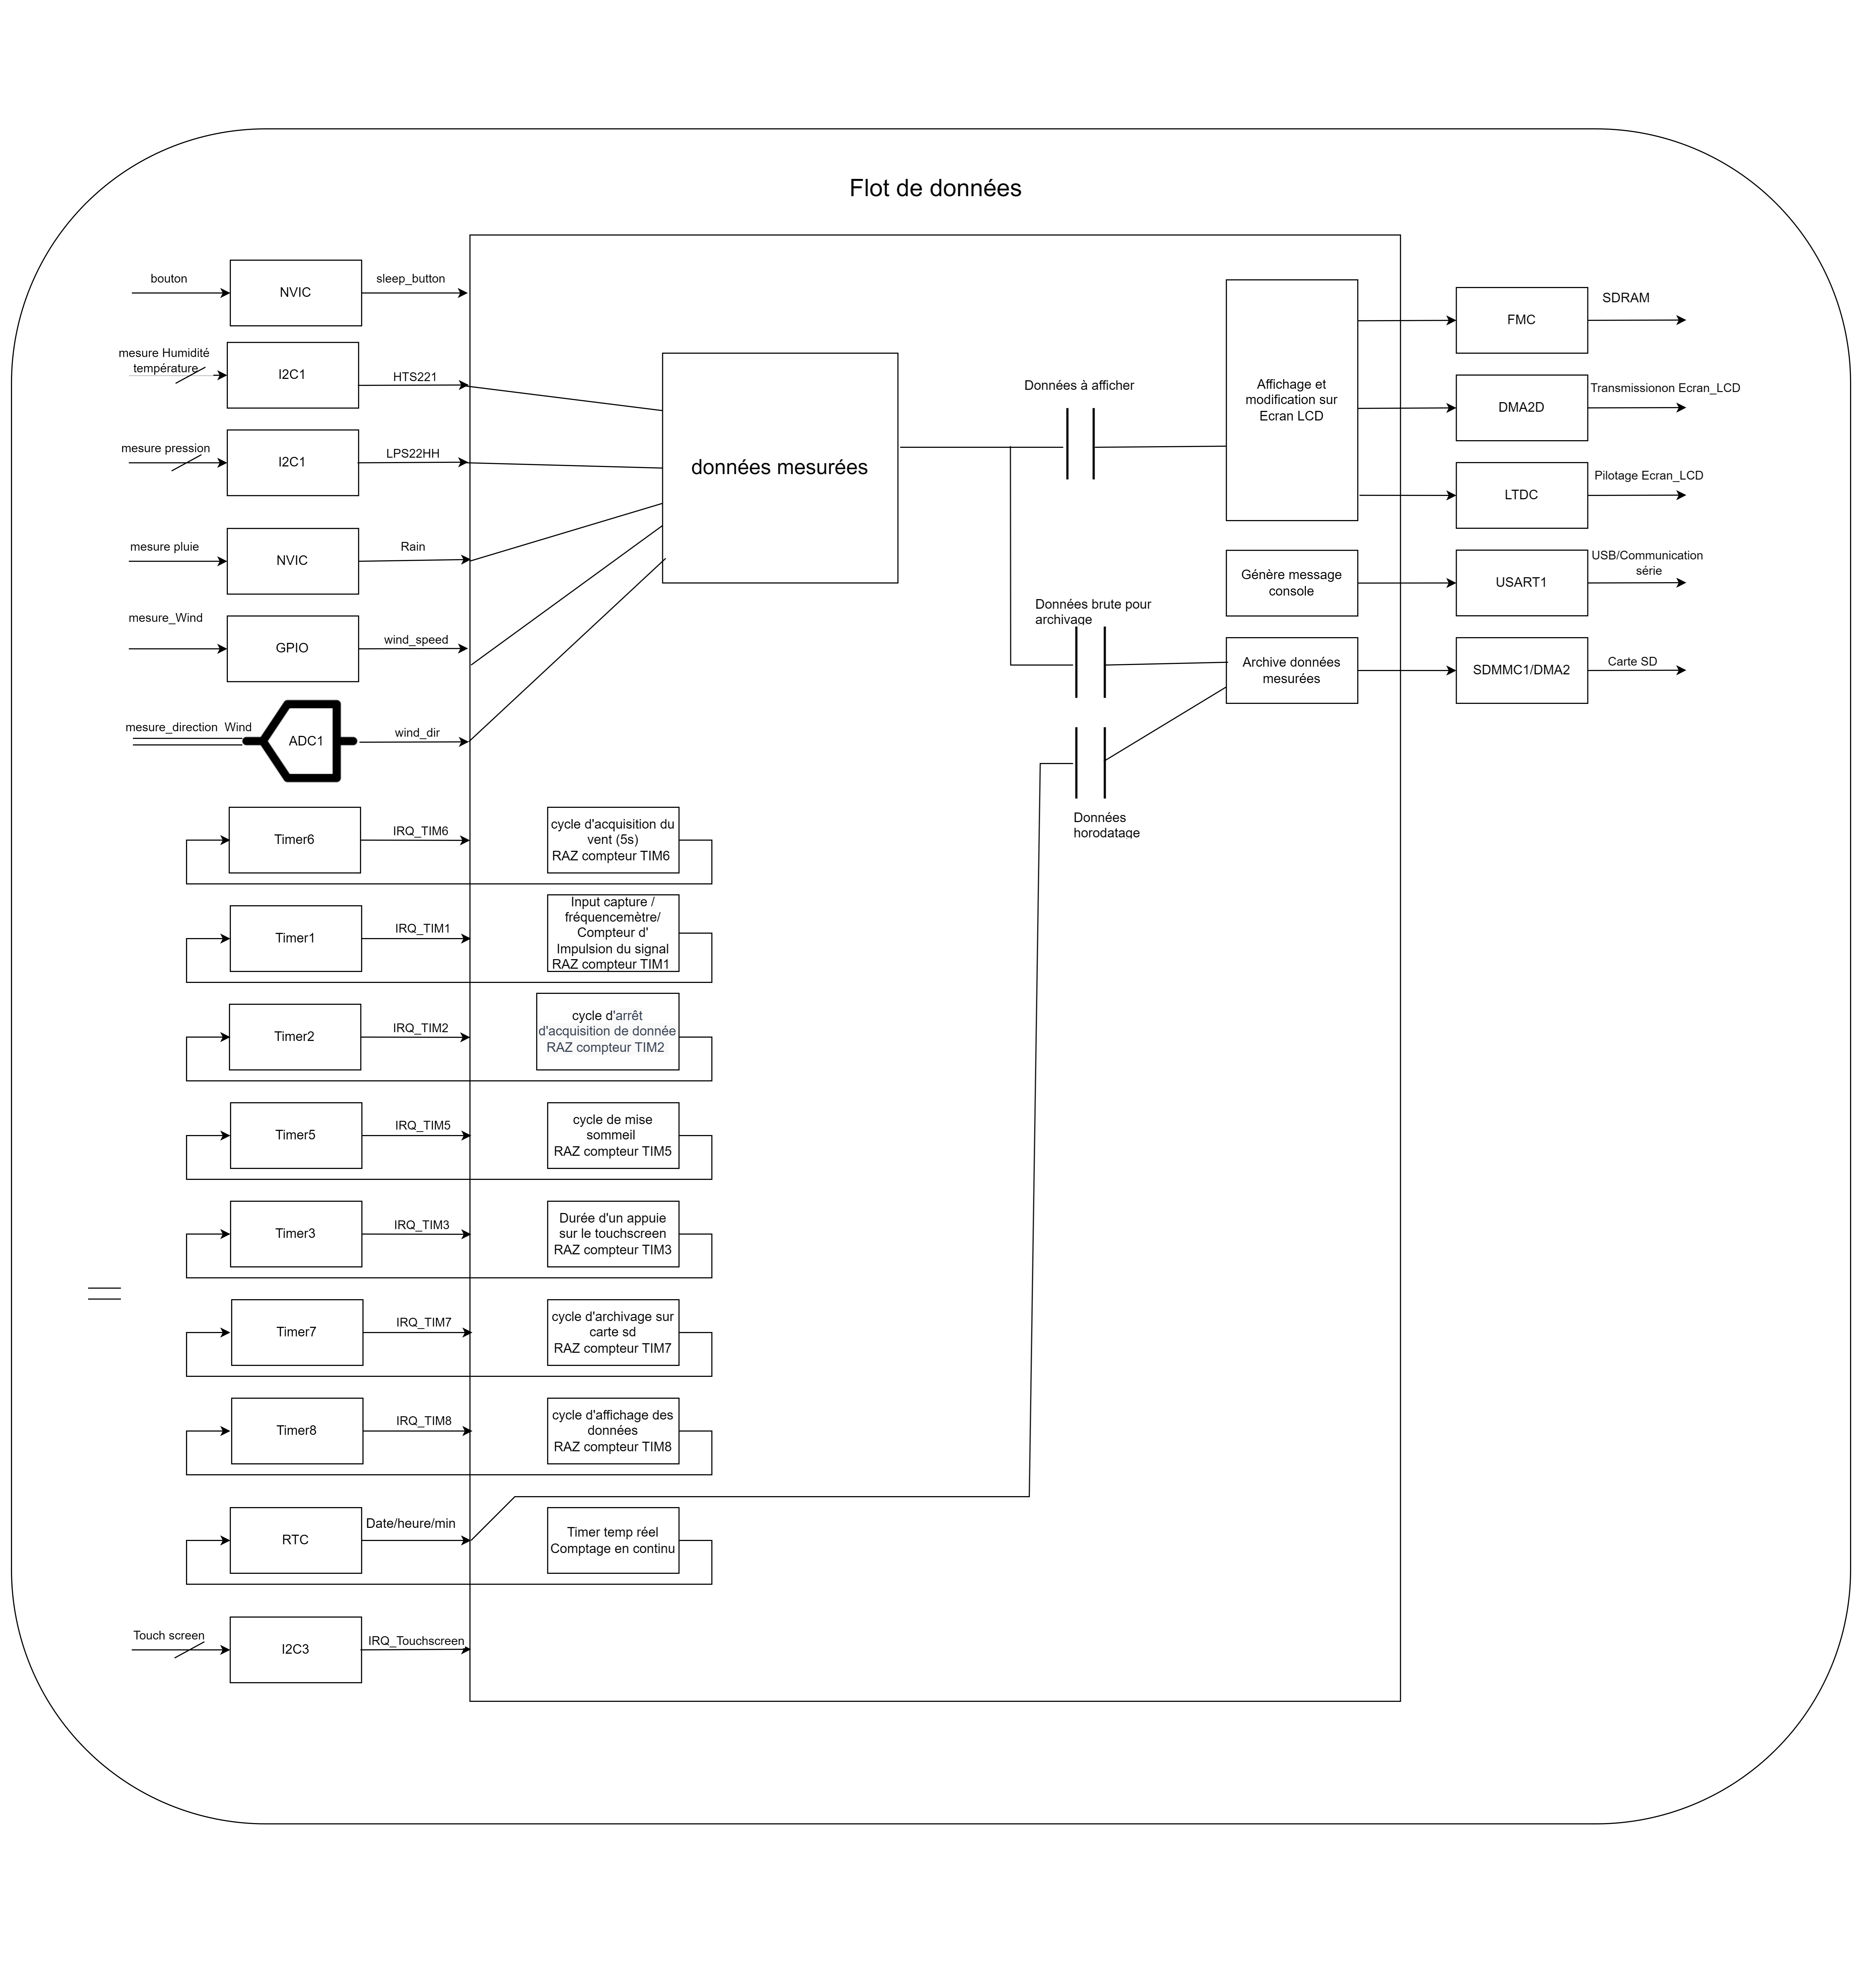
\includegraphics[width=0.8\textwidth]{./images/flot_de_donnees1.png}
    \caption{Flot de données}
    \label{fig:flot_de_donnees}
\end{figure}

Les principales transformations sont :
\begin{itemize}
    \item Acquisition des données brutes des capteurs
    \item Conversion et mise en forme des données
    \item Calcul des moyennes et statistiques
    \item Formatage pour affichage et stockage
\end{itemize}

\subsection{Diagramme de flot d'événements}
Le diagramme de flot d'événements montre la séquence des événements système :

\begin{figure}[H]
    \capstart
    \centering
    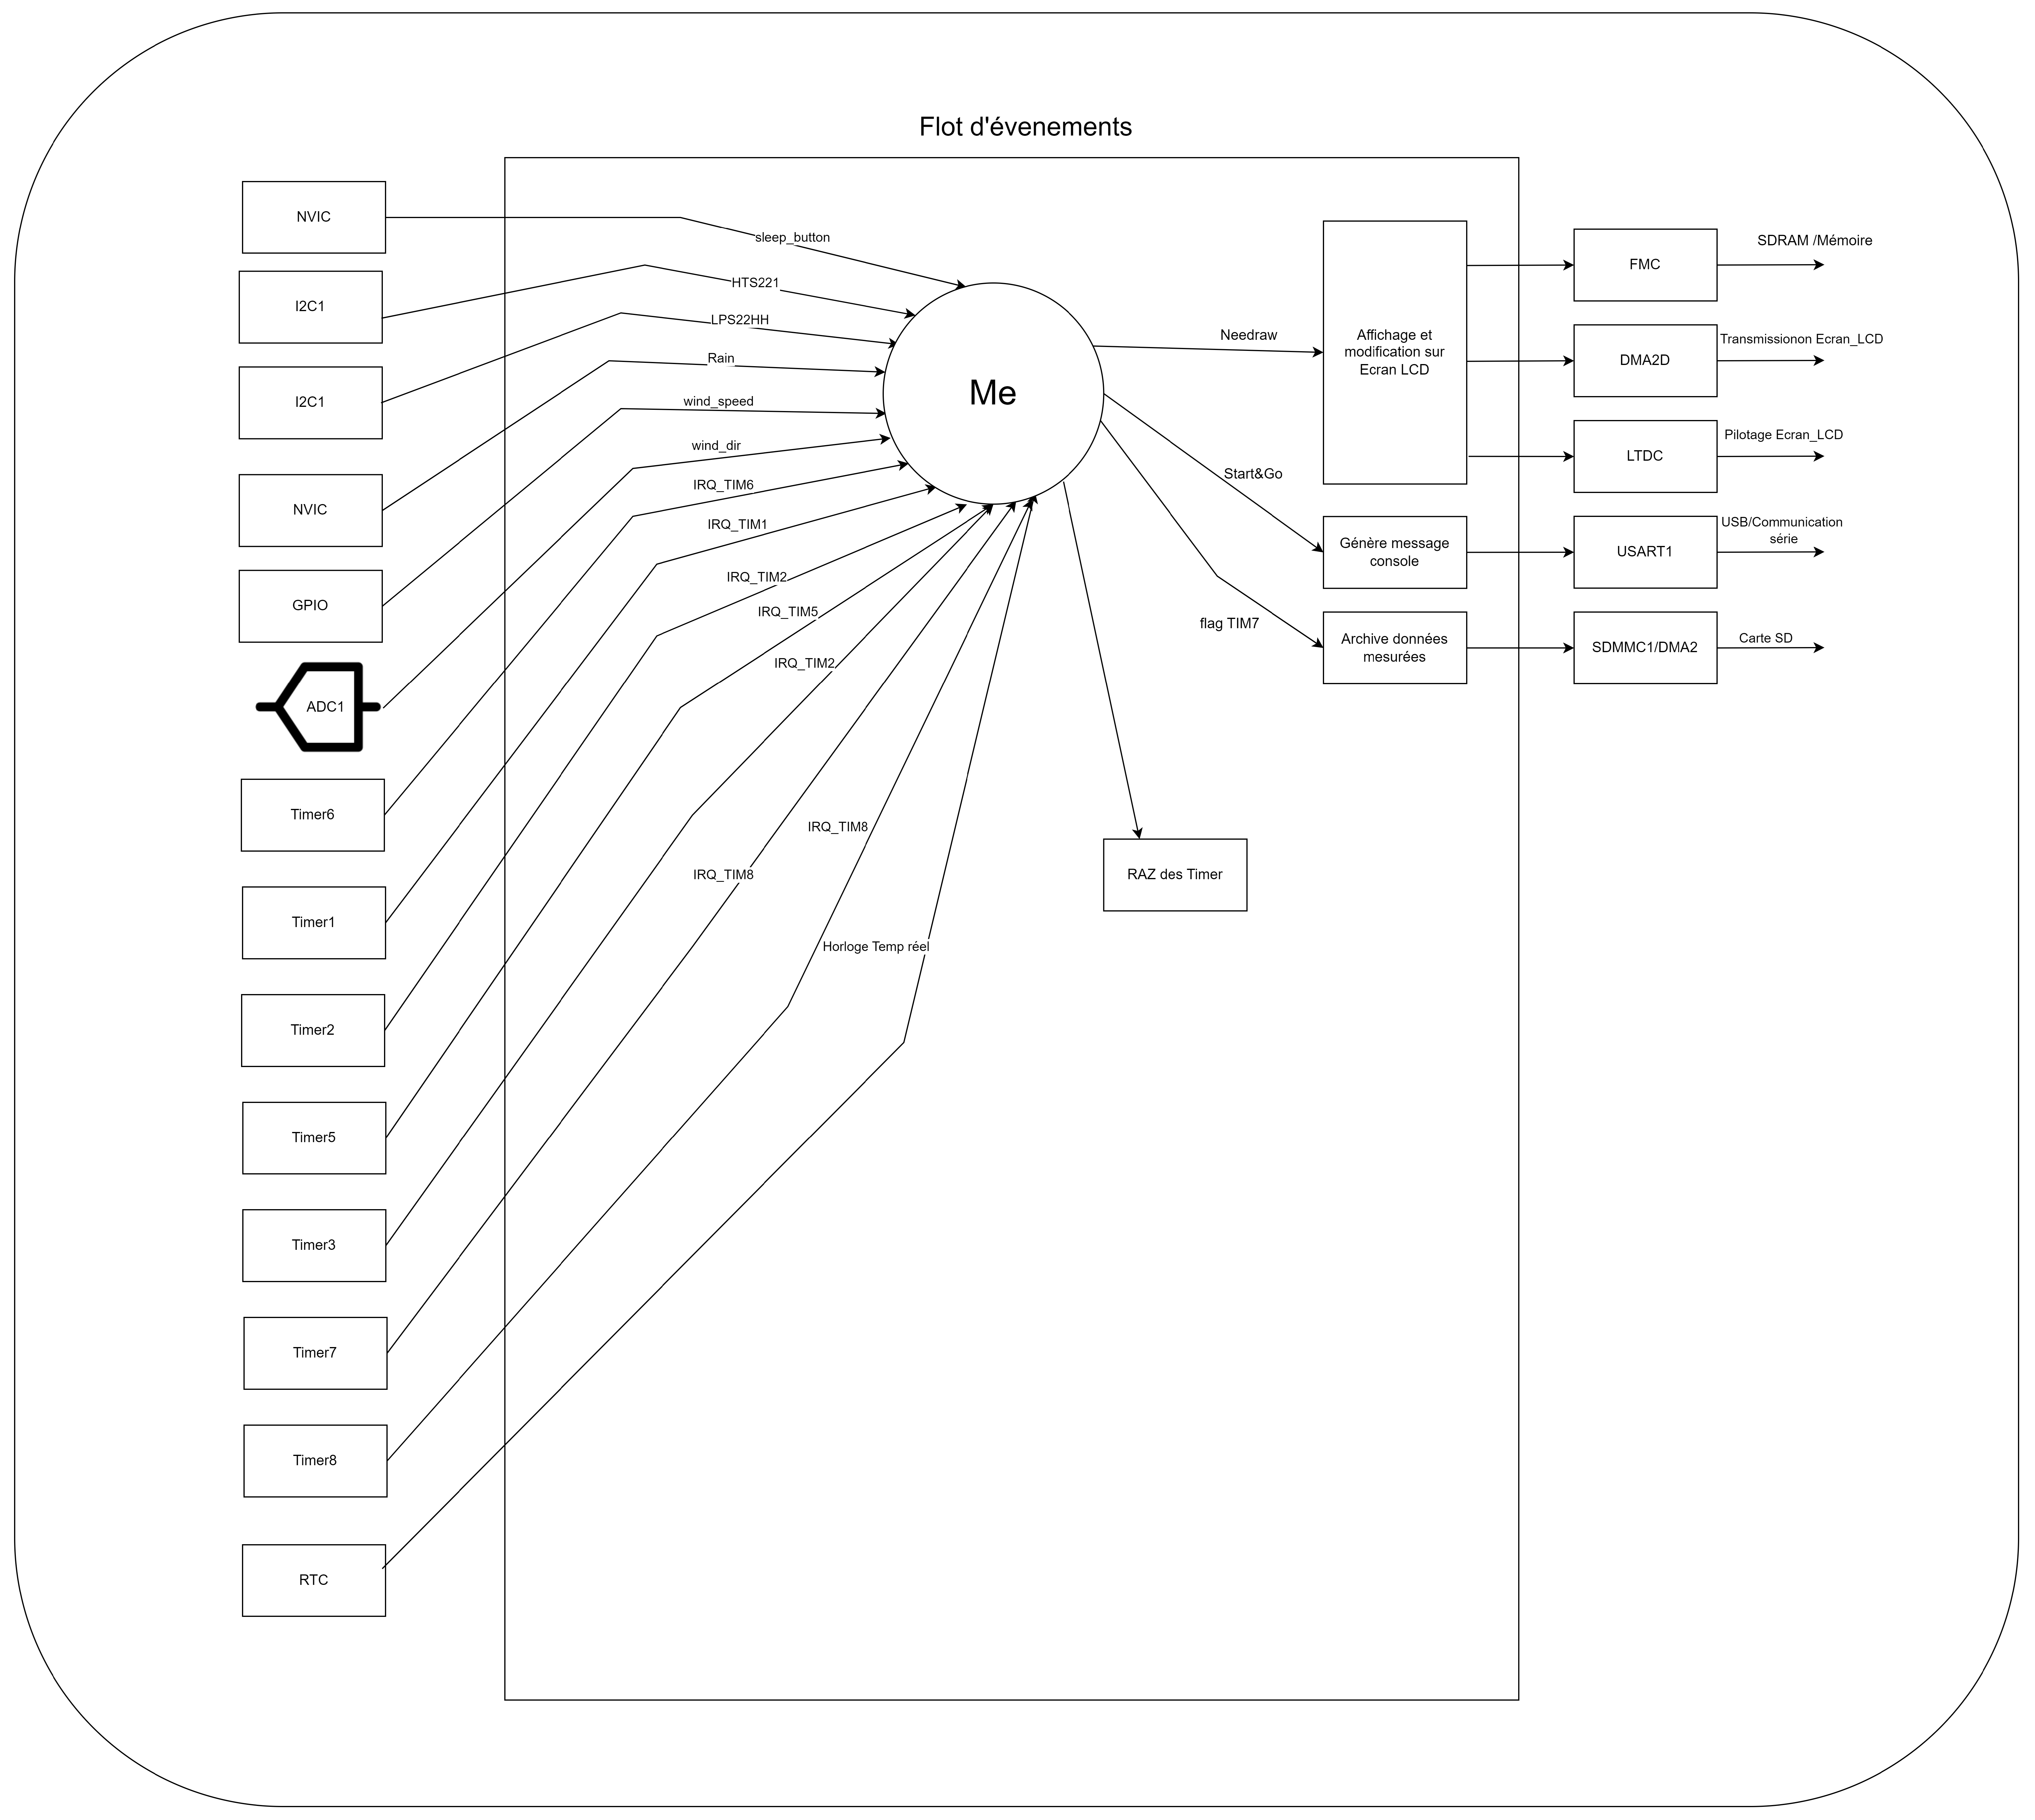
\includegraphics[width=0.8\textwidth]{./images/flot_evenements.png}
    \caption{Flot d'événements}
    \label{fig:flot_d_evenements}
\end{figure}

Les principaux événements sont :
\begin{itemize}
    \item Interruptions des capteurs à impulsions
    \item Timers d'échantillonnage
    \item Événements utilisateur (interface LCD)
    \item Événements de stockage SD
\end{itemize}

\subsection{Machine d'états / GRAFCET}
La machine d'états globale du système se présente comme suit :

\begin{figure}[H]
    \capstart
    \centering
    
\includegraphics[width=0.8\textwidth]{./images/grafcetfinal.png}
    \caption{GRAFCET Principal}
    \label{fig:grafcet_principal}
\end{figure}

Les principaux états sont :
\begin{itemize}
    \item Initialisation du système
    \item Acquisition des données
    \item Traitement et mise à jour des mesures
\end{itemize}

Les sous machines d'états sont représentées dans les diagrammes suivants :

\begin{figure}[H]
    \capstart
    \centering
    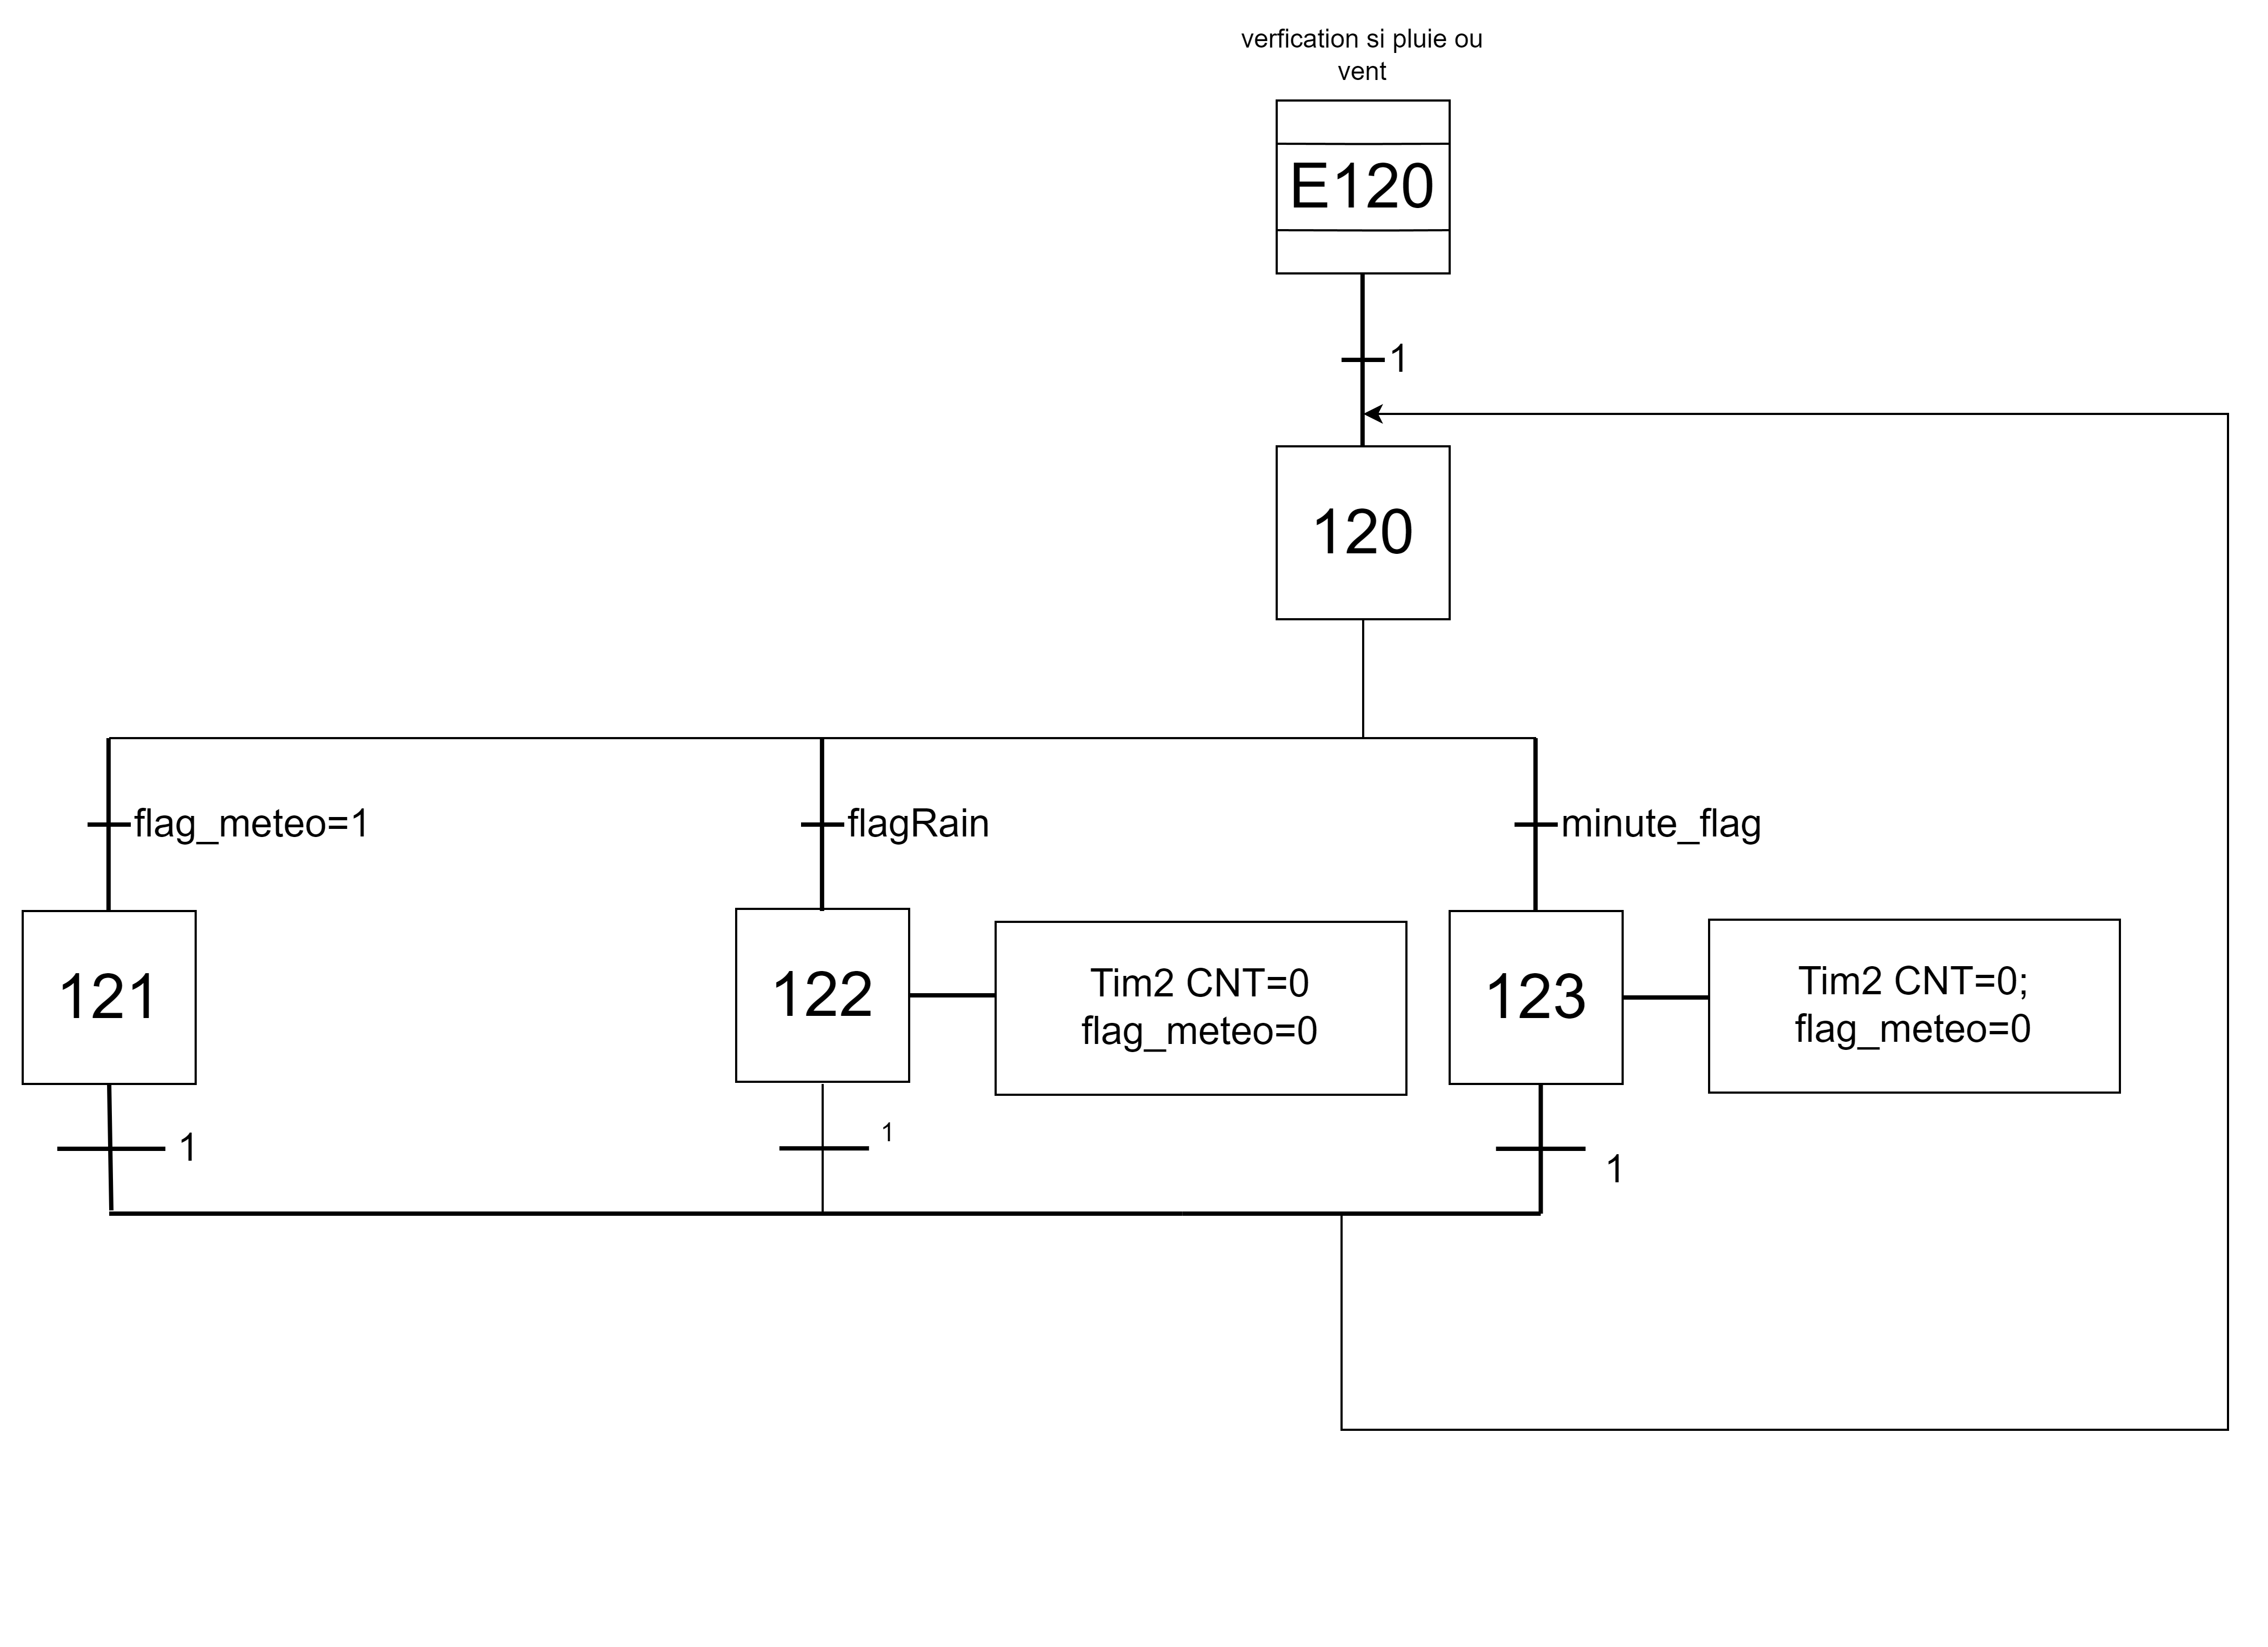
\includegraphics[width=0.8\textwidth]{./images/grafcet_pluie_vent.png}
    \caption{GRAFCET Pluie et Vent}
    \label{fig:grafcet_pluie_vent}
\end{figure}
Ce grafcet permet de gérer les interruptions des capteurs de pluie et de vent.

\begin{figure}[H]
    \capstart
    \centering
    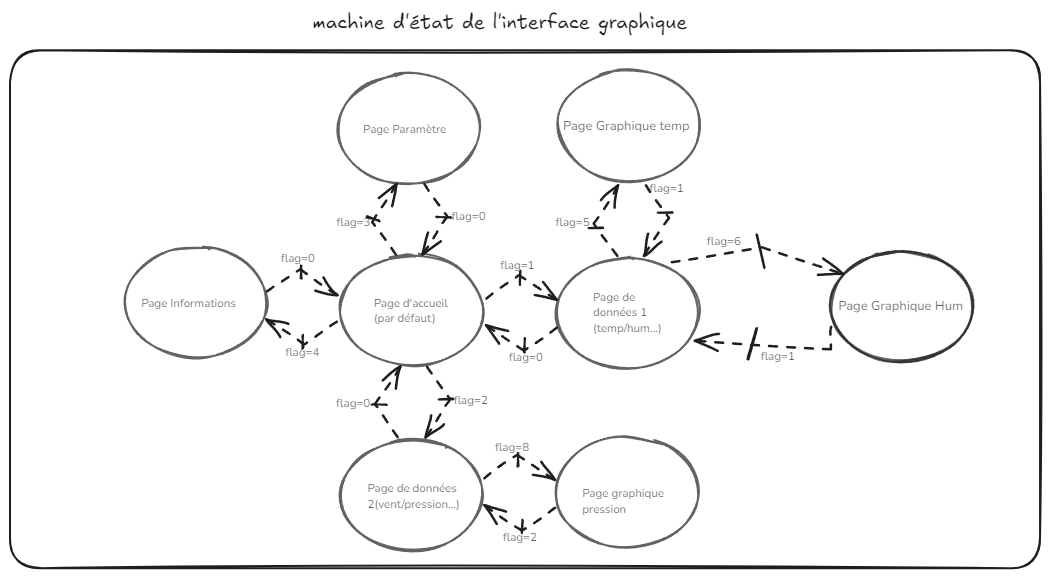
\includegraphics[width=0.8\textwidth]{./images/machine_detats_interface.png}
    \caption{Machine d'états Interface}
    \label{fig:machine_etats_interface}
\end{figure}

Ce grafcet permet de gérer les différentes pages de l'interface utilisateur.

\subsection{Table des interruptions et priorités}
\begin{table}[H]
\centering
\caption{Priorités des interruptions}
\begin{tabular}{|l|c|l|l|}
\hline
\textbf{Source} & \textbf{Priorité} & \textbf{Description} & \textbf{Fonction} \\
\hline
Timer 5 & 1 & Cycle de sommeil & Gestion mode basse consommation \\
\hline
Timer 2 & 2 & Timer périodique & Échantillonnage capteurs I2C \\
\hline
Timer 3 & 3 & Timer périodique & Rafraîchissement écran \\
\hline
Timer 8 & 4 & Timer périodique & Gestion du stockage SD \\
\hline
Timer 7 & 5 & Timer périodique & Mise à jour graphiques \\
\hline
Timer 1 \& 6 & 6 & Timer périodique & Lecture des capteurs \\
\hline
EXTI Bouton & 1 & Interruption externe & Interaction utilisateur et réveil \\
\hline
EXTI PA15 & 6 & Interruption externe & Mesure pluviométrie \\
\hline
\end{tabular}
\end{table}

Les priorités ont été définies en fonction de l'importance des tâches :
\begin{itemize}
    \item Priorité 1 : Gestion du sommeil et réveil système
    \item Priorités 2-5 : Tâches périodiques de mesure et affichage
    \item Priorité 6 : Acquisition des données des capteurs
\end{itemize}


\section{Développement et validation unitaire}

\subsection{Stratégie de test}
Avant l'intégration complète du système, chaque composant a été testé individuellement pour garantir son bon fonctionnement. Cette approche nous a permis de :
\begin{itemize}
    \item Valider le fonctionnement de chaque capteur individuellement
    \item Identifier et corriger les problèmes au plus tôt
    \item Établir une base solide pour l'intégration finale
\end{itemize}

\subsection{Capteurs environnementaux (HTS221 et LPS22HH)}
\subsubsection{Configuration}
La communication avec ces capteurs est réalisée via le bus I2C1. Voici les étapes de validation :
\begin{enumerate}
    \item Test de présence des capteurs sur le bus I2C
    \item Configuration des registres de contrôle
    \item Validation de la récupération des données
\end{enumerate}

\subsubsection{Tests réalisés}
\begin{itemize}
    \item Lecture des identifiants des capteurs
    \item Vérification de la cohérence des mesures
    \item Test de la fréquence d'échantillonnage
\end{itemize}

[Insérer capture d'écran du terminal montrant les mesures]

\subsection{Anémomètre et Girouette}
\subsubsection{Configuration matérielle}
L'anémomètre nécessite :
\begin{itemize}
    \item Une entrée GPIO configurée en interruption externe
    \item Une résistance de pull-up pour stabiliser le signal
\end{itemize}

\subsubsection{Validation}
Tests effectués à l'aide d'un vrai giroscope et d'un anémomètre :
\begin{itemize}
    \item Test des 16 positions de la girouette
\end{itemize}

\begin{figure}[H]
    \capstart
    \centering
    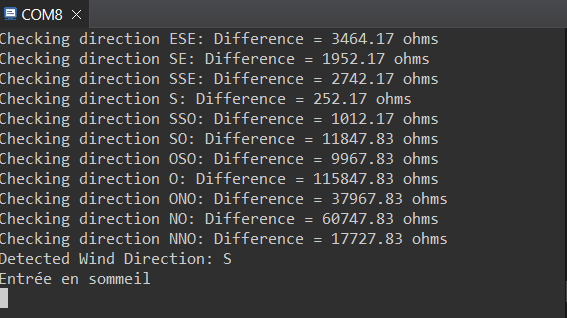
\includegraphics[width=0.8\textwidth]{./images/console_direction_du_vent_et_miseenveille.png}
    \caption{Directions du vent et mise en veille (vue de la console)} 
    \label{fig:girouette_positions}
\end{figure}

\subsection{Pluviomètre}
\subsubsection{Configuration matérielle}
Le pluviomètre de type "tipping bucket" nécessite :
\begin{itemize}
    \item Une entrée GPIO configurée en interruption externe
    \item Une résistance de pull-up interne activée
    \item Configuration de l'antirebond logiciel
\end{itemize}

\subsubsection{Tests de validation}
\begin{itemize}
    \item Test unitaire avec simulation manuelle des basculements
    \item Vérification du comptage des impulsions
    \item Validation de la conversion (0,2794 mm par basculement)
    \item Test de l'antirebond
\end{itemize}

\subsection{Interface utilisateur LCD}
\subsubsection{Configuration}
\begin{itemize}
    \item Initialisation du contrôleur LTDC
    \item Configuration de la résolution (480x272)
    \item Configuration du format de couleur (RGB565)
\end{itemize}

\subsubsection{Tests effectués}
\begin{itemize}
    \item Test d'affichage des caractères
    \item Validation du rafraîchissement de l'écran
    \item Test des différentes zones d'affichage
    \item Vérification du contraste et de la lisibilité
\end{itemize}

\begin{figure}[H]
    \capstart
    \centering
    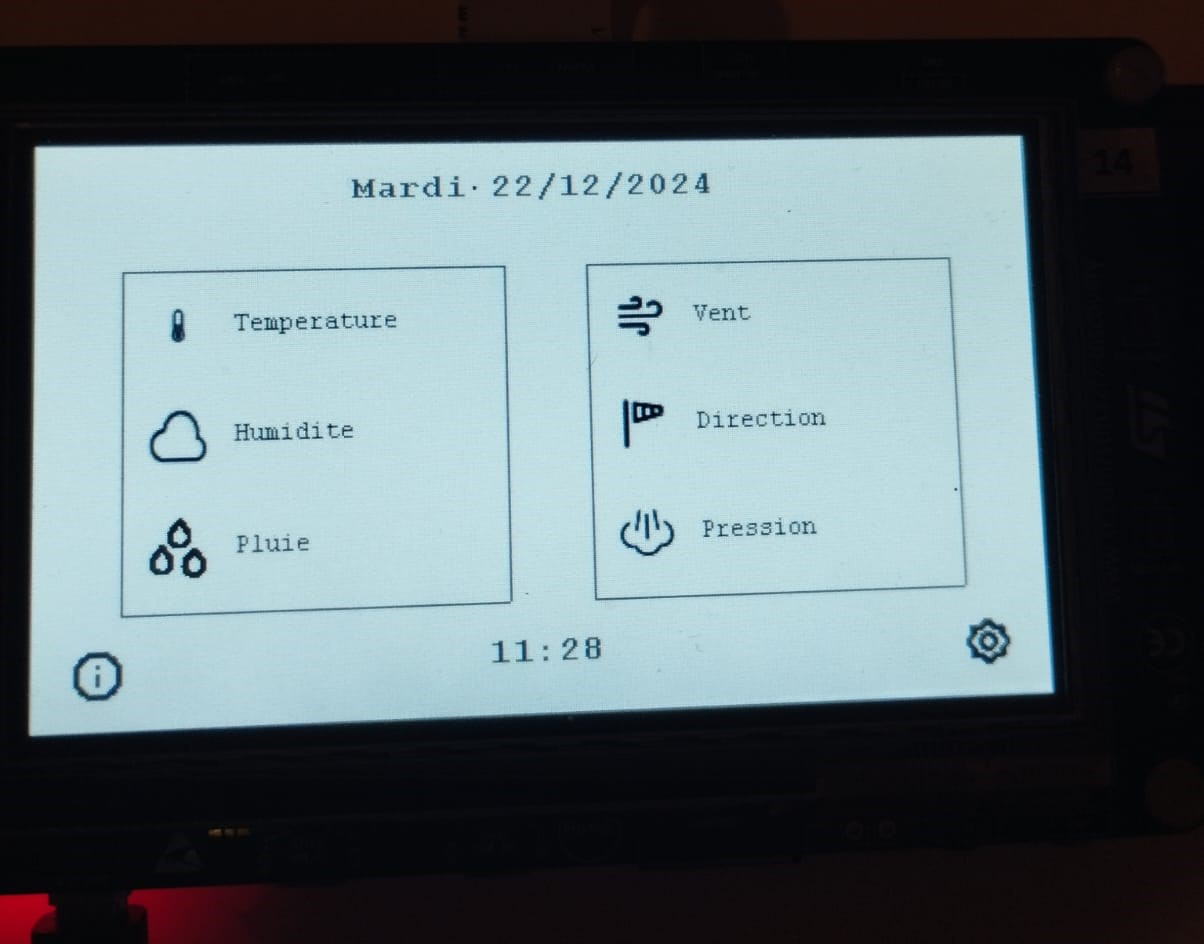
\includegraphics[width=0.8\textwidth]{./images/interface_mainpage.jpg}
    \caption{Interface utilisateur - Page principale}
    \label{fig:interface_mainpage}
\end{figure}

\subsection{Stockage sur carte SD}
\subsubsection{Configuration}
\begin{itemize}
    \item Initialisation du contrôleur SDMMC en mode 4 bits
    \item Configuration du système de fichiers FAT via FatFS
    \item Configuration du DMA pour les transferts
\end{itemize}

\subsubsection{Validation}
\begin{itemize}
    \item Test de création de fichiers
    \item Validation de l'écriture et lecture des données
    \item Test de performance en écriture continue
    \item Vérification de l'intégrité des données
\end{itemize}

[Insérer capture d'écran du contenu d'un fichier de log]


\section{Intégration et validation finale}
[À compléter]

\section{Tableau récapitulatif des fonctionnalités}

Ce tableau résume l'état de développement de chaque bloc fonctionnel du projet, ainsi que son état de validation et d'intégration.

\begin{table}[htbp]
    \centering
    \caption{État des développements et validations}
    \begin{tabular}{|p{0.25\textwidth}|p{0.2\textwidth}|p{0.2\textwidth}|p{0.2\textwidth}|}
        \hline
        \textbf{Bloc fonctionnel} & \textbf{Développement} & \textbf{Validation unitaire} & \textbf{Intégration} \\
        \hline
        \multicolumn{4}{|c|}{\textbf{Capteurs}} \\
        \hline
        Température/Humidité (HTS221) & Effectué & Validé & Intégré \\
        \hline
        Pression (LPS22HH) & Effectué & Validé & Intégré \\
        \hline
        Anémomètre & Effectué & Validé & Intégré \\
        \hline
        Girouette & Effectué & Validé & Intégré \\
        \hline
        Pluviomètre & Effectué & Validé & Intégré \\
        \hline
        \multicolumn{4}{|c|}{\textbf{Interface utilisateur}} \\
        \hline
        Écran d'accueil & Effectué & Validé & Intégré \\
        \hline
        Affichage des mesures & Effectué & Validé & Intégré \\
        \hline
        Graphiques temps réel & Effectué & Validé & Intégré \\
        \hline
        Configuration date/heure & Effectué & Validé & Intégré \\
        \hline
        \multicolumn{4}{|c|}{\textbf{Stockage}} \\
        \hline
        Gestion carte SD & Effectué & Validé & Intégré \\
        \hline
        Sauvegarde des mesures & Effectué & Validé & Intégré \\
        \hline
        \multicolumn{4}{|c|}{\textbf{Sous-parties d'assemblage}} \\
        \hline
        Agrégation des mesures & Effectué & Validé & Intégré \\
        \hline
        Gestion IHM & Effectué & Validé & Intégré \\
        \hline
        \multicolumn{4}{|c|}{\textbf{Intégration}} \\
        \hline
        Intégration finale & Effectué & Validé & Intégré \\
        \hline
    \end{tabular}
\end{table}

Le tableau ci-dessus présente :
\begin{itemize}
    \item Chaque bloc fonctionnel identifié lors de la décomposition préliminaire
    \item L'état de développement de chaque bloc
    \item Le statut de la validation unitaire
    \item L'état d'intégration dans l'application finale
    \item Les sous-parties d'assemblage et l'intégration finale
\end{itemize}


\section{Tableau récapitulatif des taches}
Ce tableau résume les tâches affectées à chaque membre de l'équipe et leur état d'avancement.

\begin{table}[htbp]
    \centering
    \resizebox{\textwidth}{!}{  % Cette ligne permet d'ajuster le tableau à la largeur de la page
        \begin{tabular}{|p{0.25\textwidth}|p{0.25\textwidth}|p{0.15\textwidth}|p{0.15\textwidth}|}
            \hline
            Nom Prénom & Tâche affectée & Tâche effectuée & Implantée version courante \\
            \hline
            Maxime MORET & Implémentation(lecture et agrégation) des capteurs I2C (Température,pluie,humidité) & Oui & Oui \\
            \hline
            Maxime MORET et Koundeme Nobel DJESSOU & Implémentation des capteurs de pluviométrie et de vent & Oui & Oui \\
            \hline
            Koundeme Nobel DJESSOU & Implémentation de l'interface utilisateur (pages de l'interface) & Oui & Oui \\
            \hline
            Koundeme Nobel DJESSOU & Implémentation de l'interaction de l'écran tactile(Partie 1) & Oui & Oui \\
            \hline
            Maxime MORET & Implémentation de l'interaction de l'écran tactile(Partie 2) & Oui & Oui \\
            \hline
            Koundeme Nobel DJESSOU & Implémentation de la RTC & Oui & Oui \\
            \hline
            Koundeme Nobel DJESSOU & Implémentation de la carte SD & Oui & Oui \\
            \hline
            Tristan GROUSSARD & Schématisation Flow de données,Flow d'événements et GRAFCET & Oui & Oui \\
            \hline
        \end{tabular}
    }
    \caption{Tâches affectées et effectuées}
    \label{table:2}
\end{table}
\newpage
\nsection{Conclusion}
Ce projet a été d'une grande richesse en termes d'apprentissage. Il nous a permis de mettre en pratique les connaissances acquises en cours de systèmes embarqués. Nous avons pu découvrir les différentes étapes de la conception d'un système embarqué, de la spécification des besoins à la réalisation du système en passant par la conception et la programmation.
\end{document}